% Generated by experiments/exp2_thesis/make_assets.py -- do not edit by hand.
\begin{figure}[tbp]
  \centering
  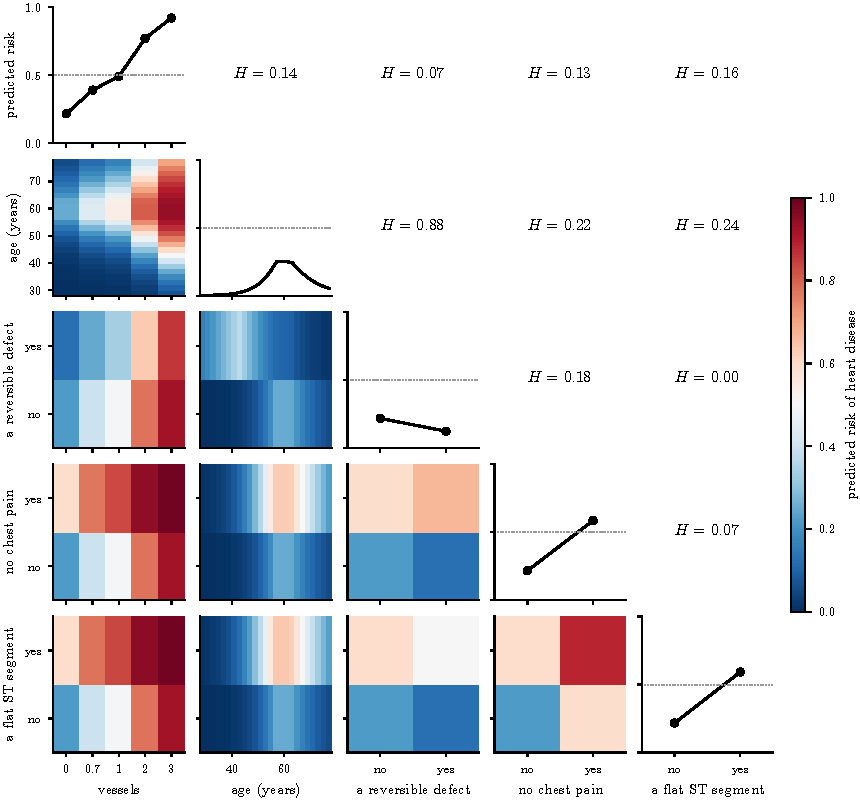
\includegraphics[width=0.95\textwidth]{figures/exp2/exp2-heart-pairs}
  \caption{Heart-100 seed 2, the whole model: a pairs plot over the five inputs it is most sensitive to. Diagonal: predicted risk as one input varies; below the diagonal: as two vary together (colour, centred on a risk of 0.5); other inputs held at their training median, which is a reference patient with a predicted risk of 0.22. Above the diagonal: the strength of each pair's interaction ($H$, the share of the pair's variation not explained by the two inputs separately, weighted by where the data lie). The strongest is age with a reversible defect.}
  \label{fig:exp2-heart-pairs}
\end{figure}
